\renewcommand{\theHfigure}{B.\arabic{figure}}

\section*{Приложение Б. Графическое исследование семи уравнений}\label{app:b}

\renewcommand{\thefigure}{Б.\arabic{figure}}\setcounter{figure}{0}

Рисунки используют только сохранённые численные ответы. Густые линии коэффициентов и точного решения вычислены по известным аналитическим формулам; численные решения существуют лишь в 33 узлах. Отрезки между их маркерами служат для чтения. Везде показан коэффициент $c$ исходного уравнения, а не $c_R$.

\subsection*{Б.1. Пример 1}\label{app:graphs1}

Полная дифференциальная постановка и числовые результаты приведены в п.~А.1. Сначала сопоставлены коэффициенты и точное решение на носителе.

\begin{center}\begin{minipage}{\linewidth}\centering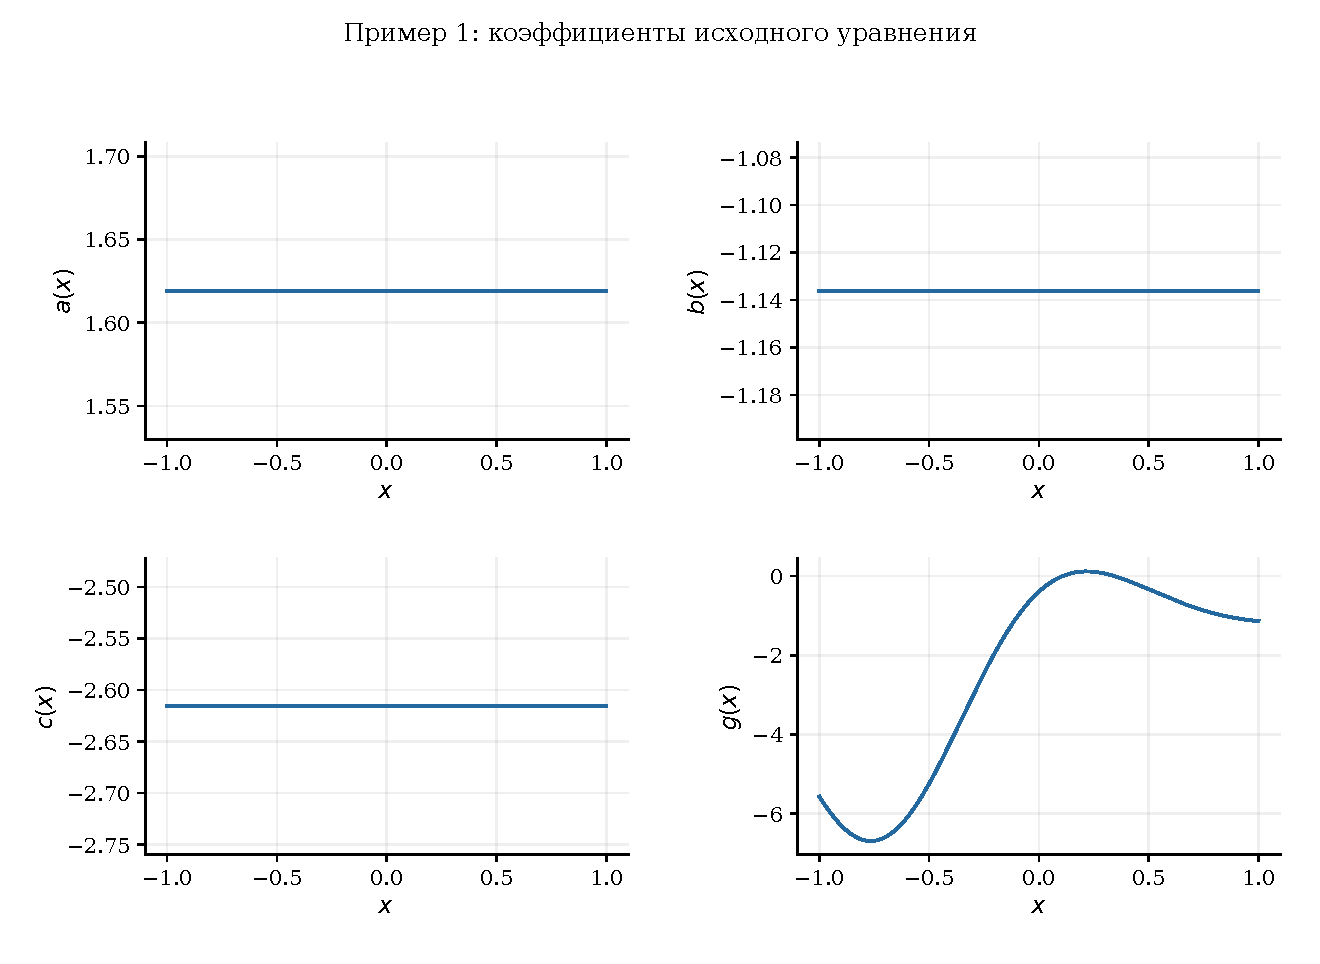
\includegraphics[width=.80\linewidth]{figures/example_01_coefficients.pdf}\captionof{figure}{Пример 1. Коэффициенты исходного уравнения на отрезке сравнения. Показан c(x), а не коэффициент $c_R(x)$ оператора. Все функции вычислены по сохранённым аналитическим определениям.}\label{fig:example_01_coefficients}\end{minipage}\end{center}

\begin{center}\begin{minipage}{\linewidth}\centering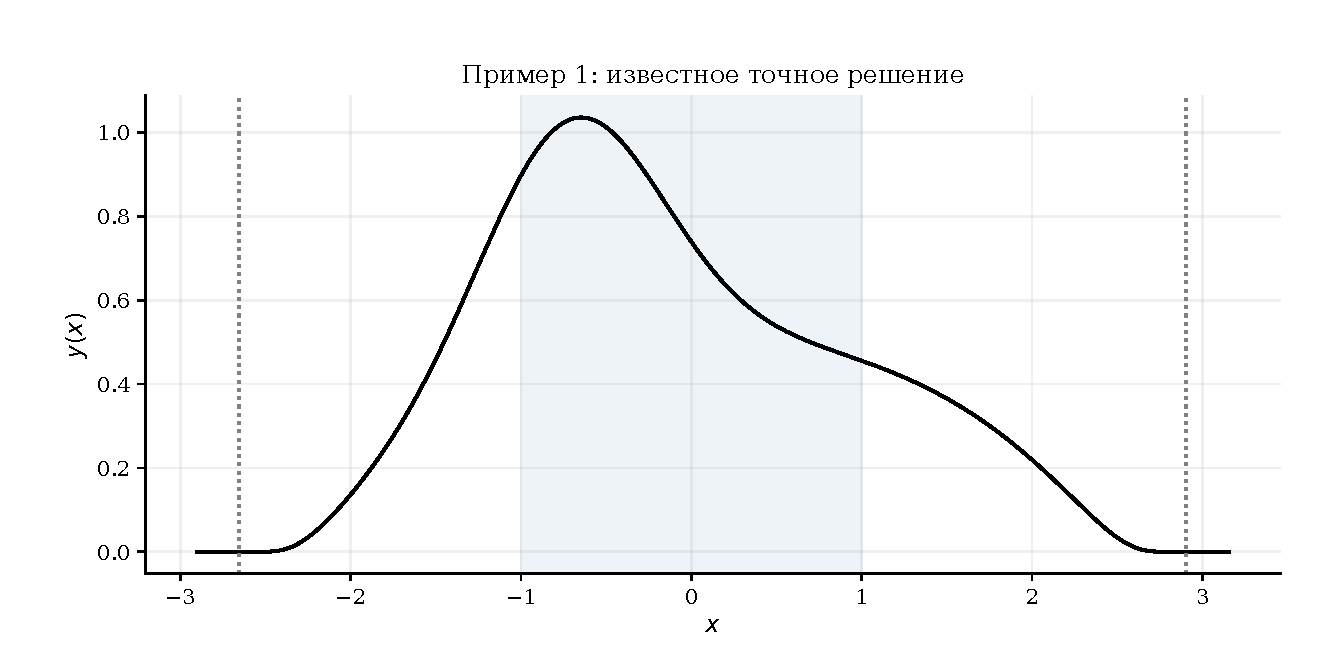
\includegraphics[width=.80\linewidth]{figures/example_01_exact.pdf}\captionof{figure}{Пример 1. Аналитическое решение на носителе и прилегающих участках прямой. Закрашен отрезок $[-1,1]$, на котором сохранены численные решения; пунктиром отмечены границы носителя.}\label{fig:example_01_exact}\end{minipage}\end{center}

\clearpage

\noindent\textbf{Пример 1: численное приближение и его ошибка.}

Кривые решений на общем масштабе могут казаться совпадающими, поэтому ниже отдельно показана абсолютная ошибка; критерием является её максимум, а не видимое совпадение отдельных участков.

\begin{center}\begin{minipage}{\linewidth}\centering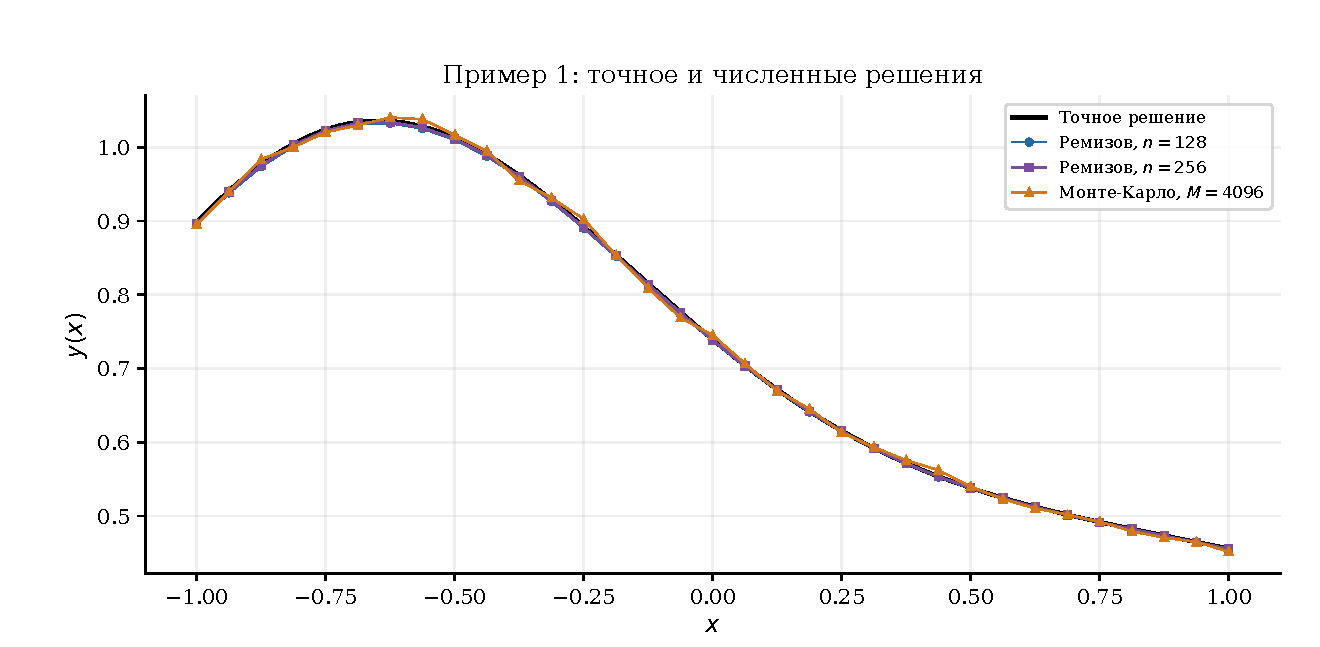
\includegraphics[width=.94\linewidth]{figures/example_01_solutions.pdf}\captionof{figure}{Пример 1. Точная кривая и сохранённые значения численных решений в 33 узлах. Отрезки между маркерами служат только для чтения. Новые численные значения между узлами не рассчитывались.}\label{fig:example_01_solutions}\end{minipage}\end{center}

\begin{center}\begin{minipage}{\linewidth}\centering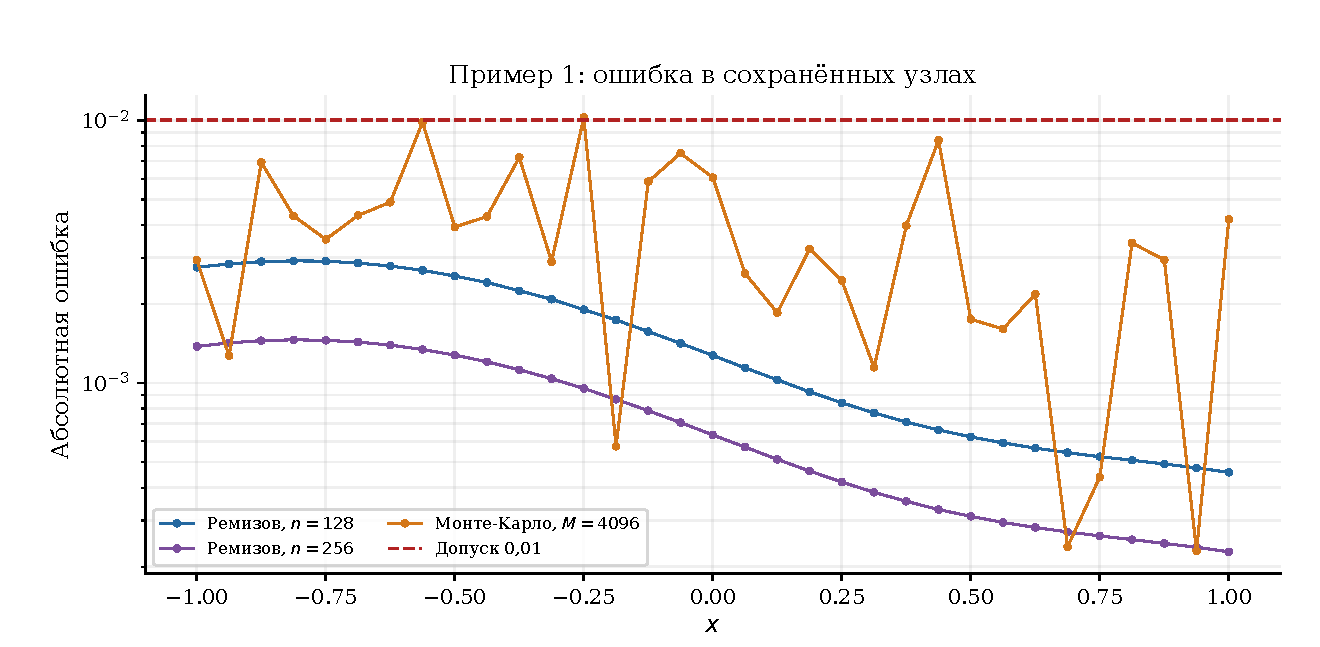
\includegraphics[width=.94\linewidth]{figures/example_01_error.pdf}\captionof{figure}{Пример 1. Абсолютная ошибка по сохранённым численным значениям. Порог относится к максимуму по 33 узлам; поведение ошибки между узлами не установлено.}\label{fig:example_01_error}\end{minipage}\end{center}

\clearpage

\subsection*{Б.2. Пример 2}\label{app:graphs2}

Полная дифференциальная постановка и числовые результаты приведены в п.~А.2. Сначала сопоставлены коэффициенты и точное решение на носителе.

\begin{center}\begin{minipage}{\linewidth}\centering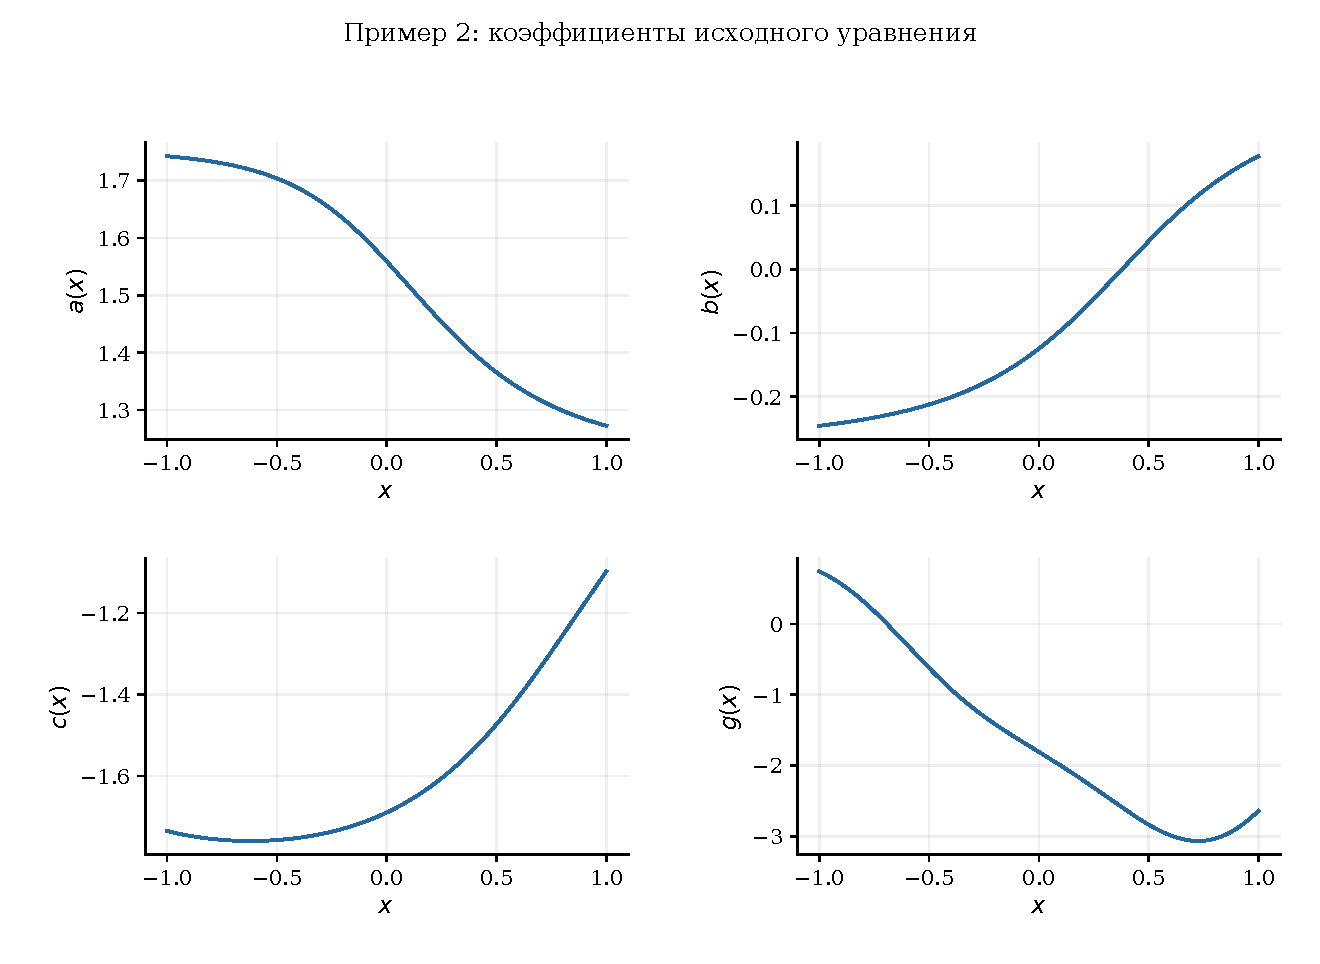
\includegraphics[width=.94\linewidth]{figures/example_02_coefficients.pdf}\captionof{figure}{Пример 2. Коэффициенты исходного уравнения на отрезке сравнения. Показан c(x), а не коэффициент $c_R(x)$ оператора. Все функции вычислены по сохранённым аналитическим определениям.}\label{fig:example_02_coefficients}\end{minipage}\end{center}

\begin{center}\begin{minipage}{\linewidth}\centering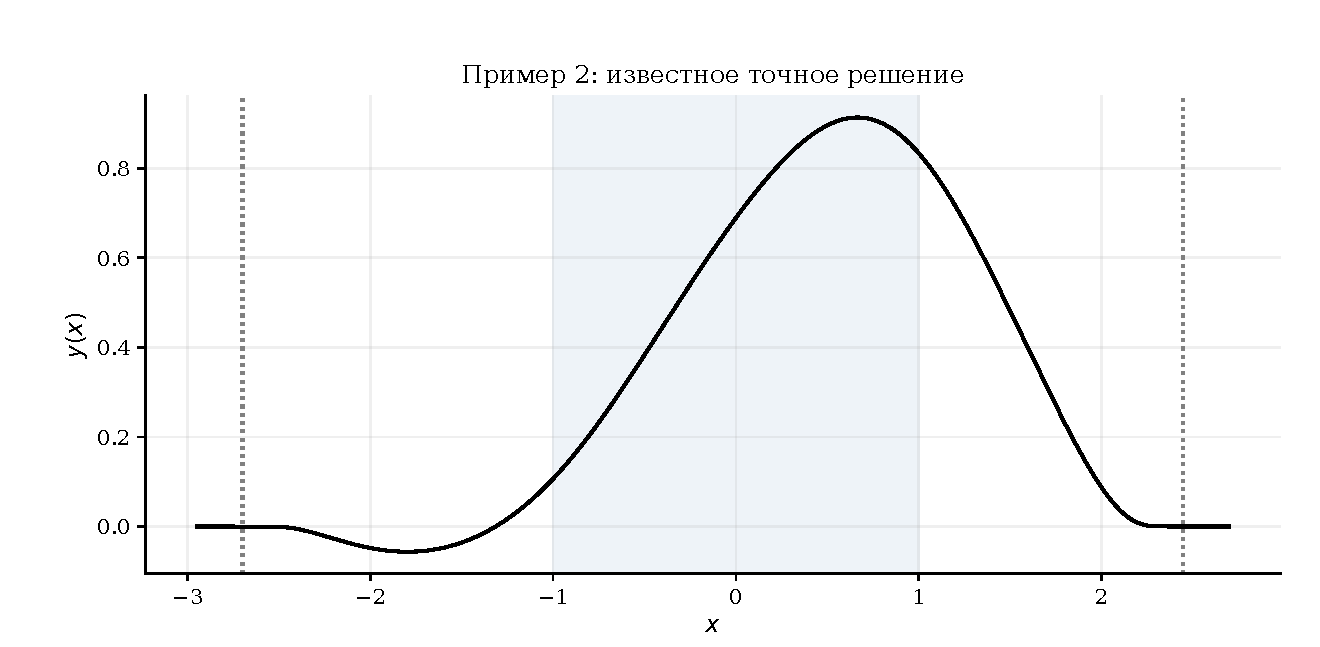
\includegraphics[width=.94\linewidth]{figures/example_02_exact.pdf}\captionof{figure}{Пример 2. Аналитическое решение на носителе и прилегающих участках прямой. Закрашен отрезок $[-1,1]$, на котором сохранены численные решения; пунктиром отмечены границы носителя.}\label{fig:example_02_exact}\end{minipage}\end{center}

\clearpage

\noindent\textbf{Пример 2: численное приближение и его ошибка.}

Кривые решений на общем масштабе могут казаться совпадающими, поэтому ниже отдельно показана абсолютная ошибка; критерием является её максимум, а не видимое совпадение отдельных участков.

\begin{center}\begin{minipage}{\linewidth}\centering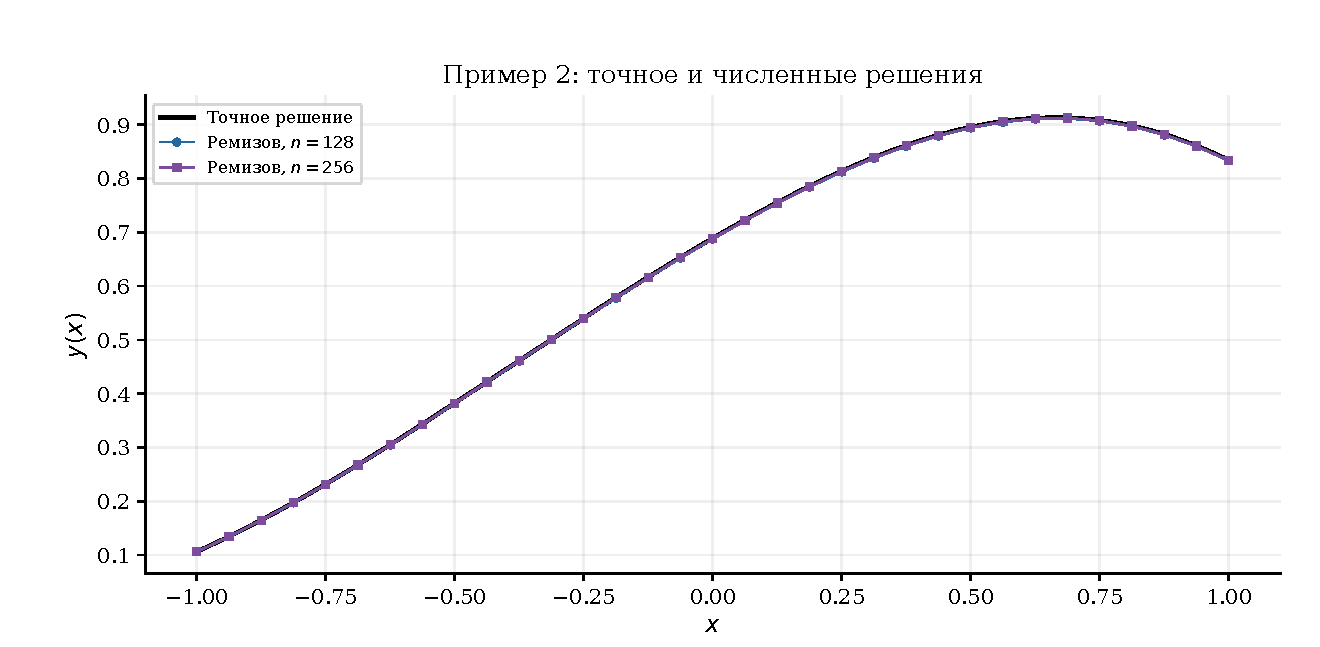
\includegraphics[width=.94\linewidth]{figures/example_02_solutions.pdf}\captionof{figure}{Пример 2. Точная кривая и сохранённые значения численных решений в 33 узлах. Отрезки между маркерами служат только для чтения. Новые численные значения между узлами не рассчитывались.}\label{fig:example_02_solutions}\end{minipage}\end{center}

\begin{center}\begin{minipage}{\linewidth}\centering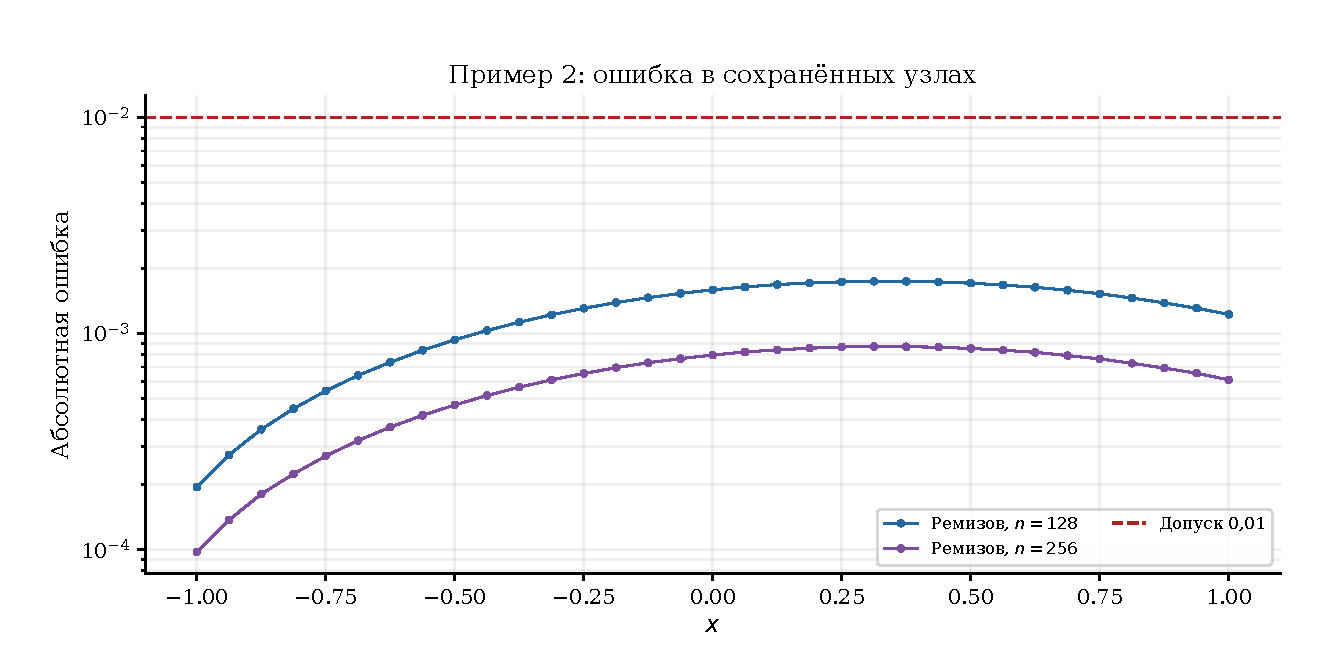
\includegraphics[width=.94\linewidth]{figures/example_02_error.pdf}\captionof{figure}{Пример 2. Абсолютная ошибка по сохранённым численным значениям. Порог относится к максимуму по 33 узлам; поведение ошибки между узлами не установлено.}\label{fig:example_02_error}\end{minipage}\end{center}

\clearpage

\subsection*{Б.3. Пример 3}\label{app:graphs3}

Полная дифференциальная постановка и числовые результаты приведены в п.~А.3. Сначала сопоставлены коэффициенты и точное решение на носителе.

\begin{center}\begin{minipage}{\linewidth}\centering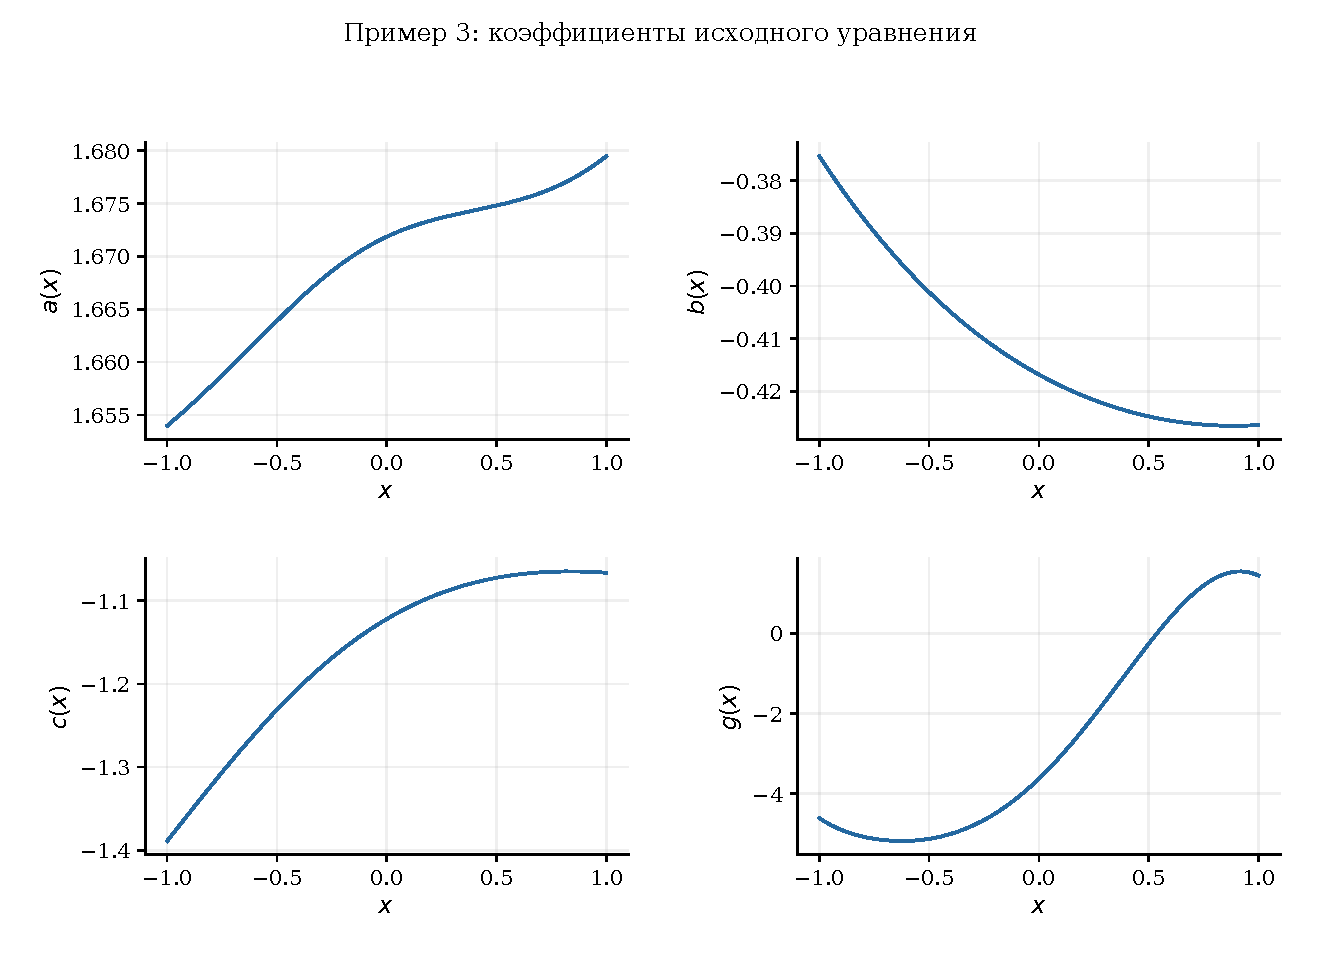
\includegraphics[width=.94\linewidth]{figures/example_03_coefficients.pdf}\captionof{figure}{Пример 3. Коэффициенты исходного уравнения на отрезке сравнения. Показан c(x), а не коэффициент $c_R(x)$ оператора. Все функции вычислены по сохранённым аналитическим определениям.}\label{fig:example_03_coefficients}\end{minipage}\end{center}

\begin{center}\begin{minipage}{\linewidth}\centering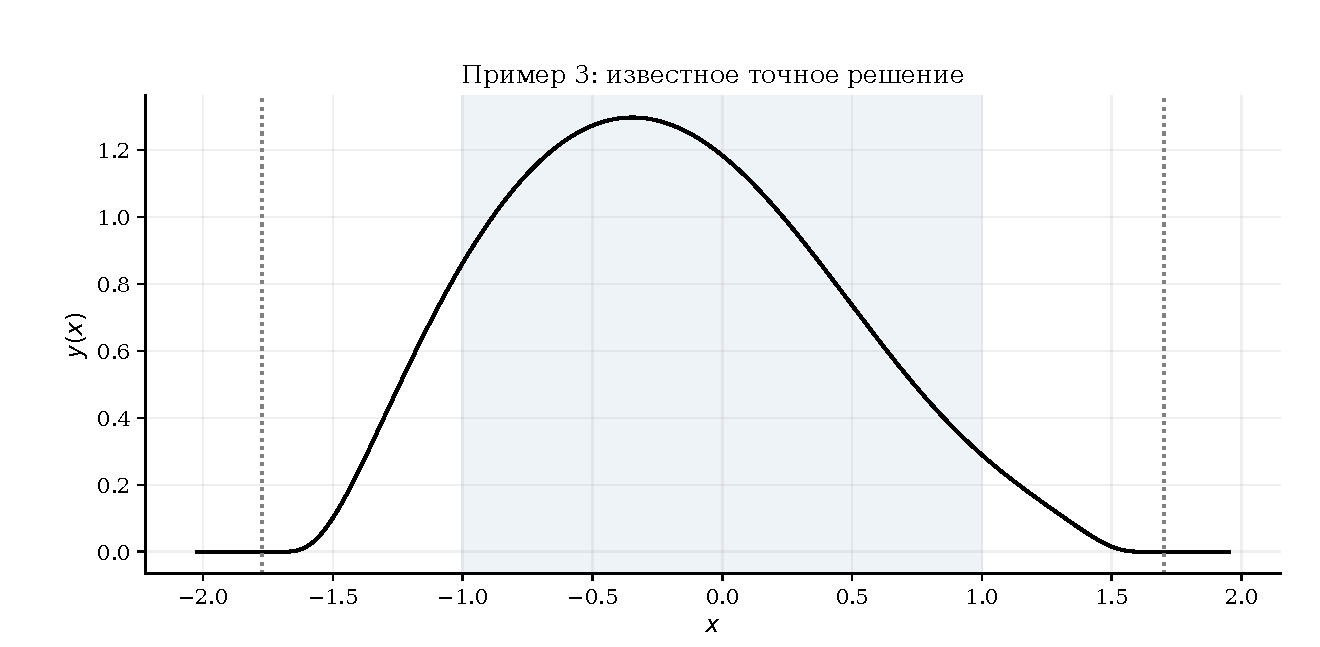
\includegraphics[width=.94\linewidth]{figures/example_03_exact.pdf}\captionof{figure}{Пример 3. Аналитическое решение на носителе и прилегающих участках прямой. Закрашен отрезок $[-1,1]$, на котором сохранены численные решения; пунктиром отмечены границы носителя.}\label{fig:example_03_exact}\end{minipage}\end{center}

\clearpage

\noindent\textbf{Пример 3: численное приближение и его ошибка.}

Кривые решений на общем масштабе могут казаться совпадающими, поэтому ниже отдельно показана абсолютная ошибка; критерием является её максимум, а не видимое совпадение отдельных участков.

\begin{center}\begin{minipage}{\linewidth}\centering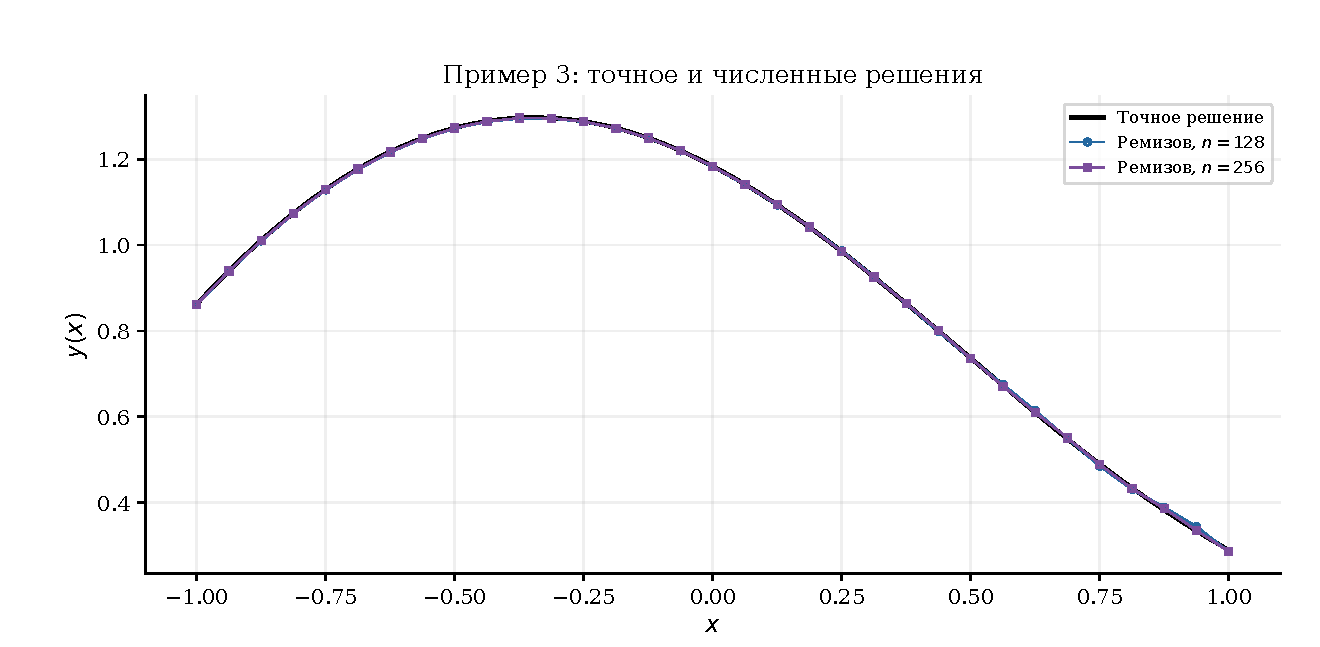
\includegraphics[width=.94\linewidth]{figures/example_03_solutions.pdf}\captionof{figure}{Пример 3. Точная кривая и сохранённые значения численных решений в 33 узлах. Отрезки между маркерами служат только для чтения. Новые численные значения между узлами не рассчитывались.}\label{fig:example_03_solutions}\end{minipage}\end{center}

\begin{center}\begin{minipage}{\linewidth}\centering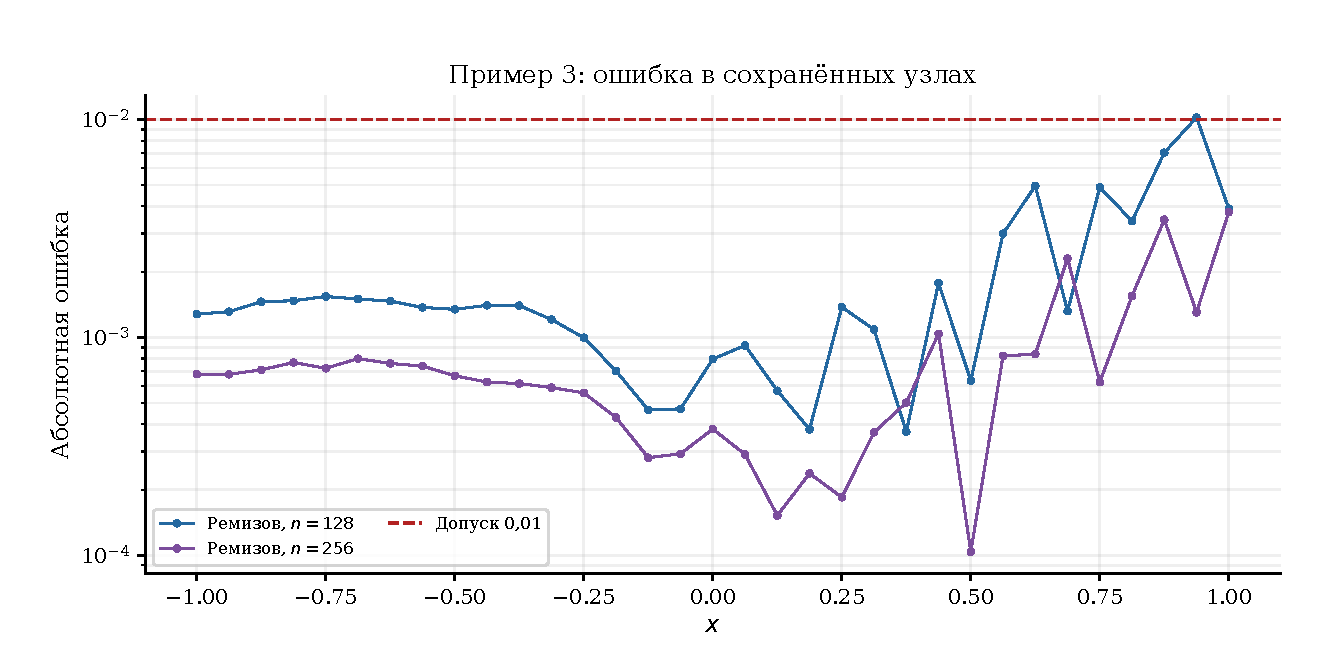
\includegraphics[width=.94\linewidth]{figures/example_03_error.pdf}\captionof{figure}{Пример 3. Абсолютная ошибка по сохранённым численным значениям. Порог относится к максимуму по 33 узлам; поведение ошибки между узлами не установлено.}\label{fig:example_03_error}\end{minipage}\end{center}

\clearpage

\subsection*{Б.4. Пример 4}\label{app:graphs4}

Полная дифференциальная постановка и числовые результаты приведены в п.~А.4. Сначала сопоставлены коэффициенты и точное решение на носителе.

\begin{center}\begin{minipage}{\linewidth}\centering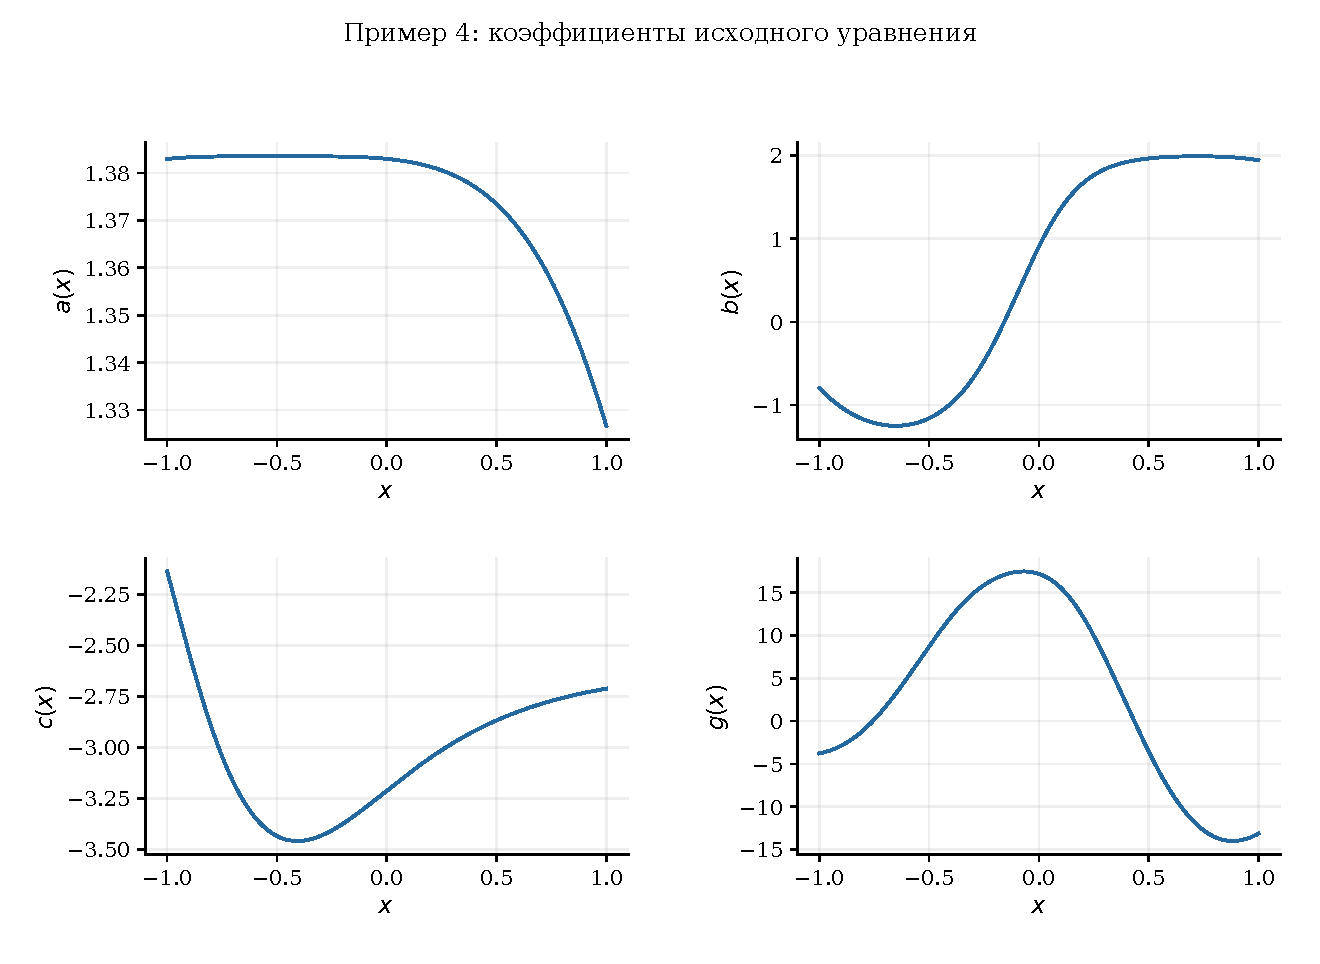
\includegraphics[width=.94\linewidth]{figures/example_04_coefficients.pdf}\captionof{figure}{Пример 4. Коэффициенты исходного уравнения на отрезке сравнения. Показан c(x), а не коэффициент $c_R(x)$ оператора. Все функции вычислены по сохранённым аналитическим определениям.}\label{fig:example_04_coefficients}\end{minipage}\end{center}

\begin{center}\begin{minipage}{\linewidth}\centering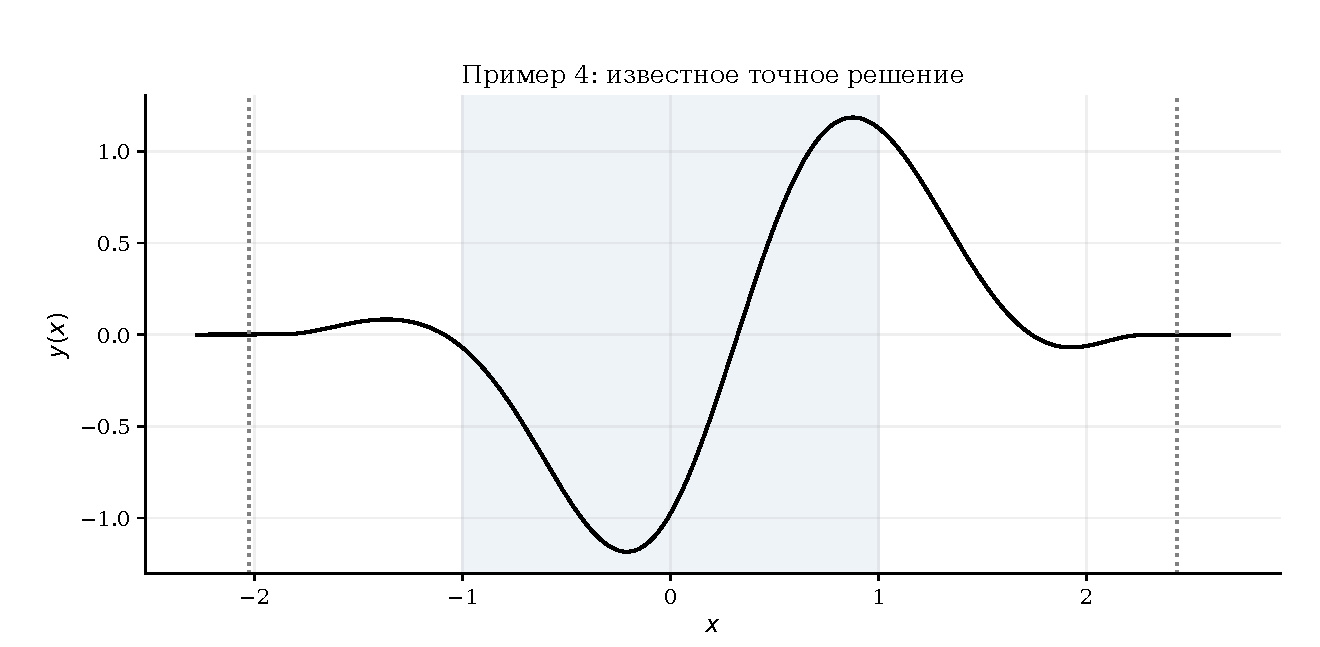
\includegraphics[width=.94\linewidth]{figures/example_04_exact.pdf}\captionof{figure}{Пример 4. Аналитическое решение на носителе и прилегающих участках прямой. Закрашен отрезок $[-1,1]$, на котором сохранены численные решения; пунктиром отмечены границы носителя.}\label{fig:example_04_exact}\end{minipage}\end{center}

\clearpage

\noindent\textbf{Пример 4: численное приближение и его ошибка.}

Кривые решений на общем масштабе могут казаться совпадающими, поэтому ниже отдельно показана абсолютная ошибка; критерием является её максимум, а не видимое совпадение отдельных участков.

\begin{center}\begin{minipage}{\linewidth}\centering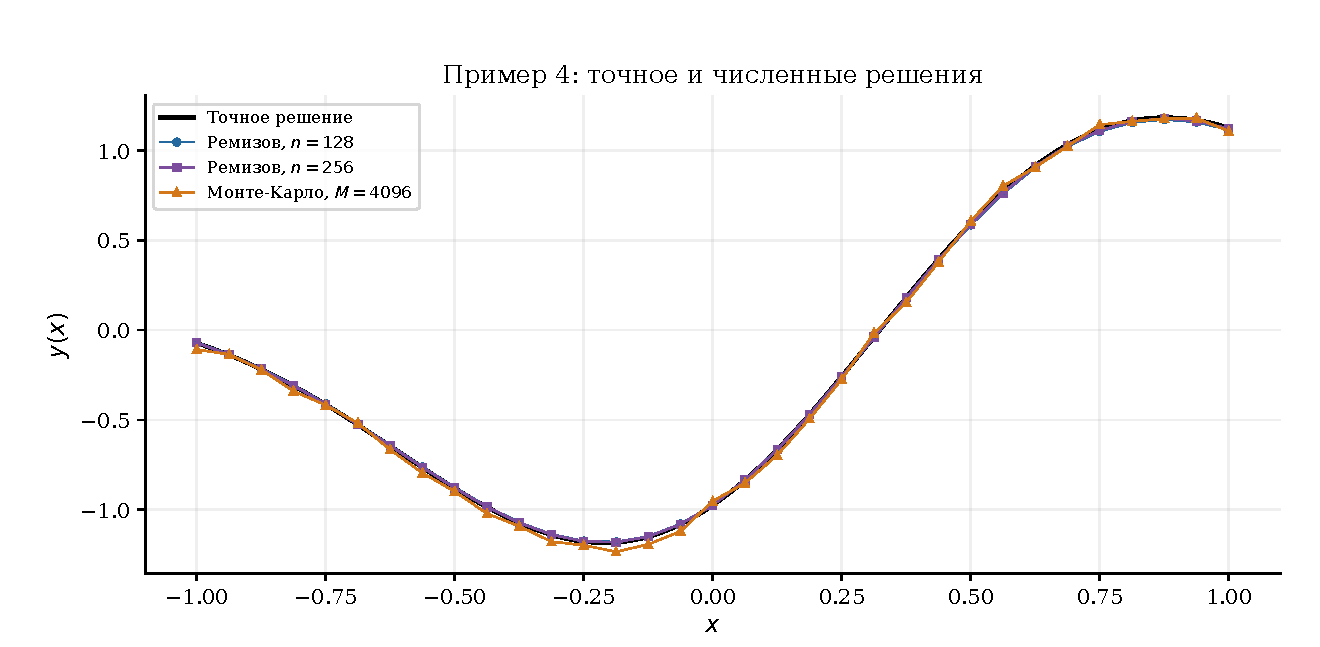
\includegraphics[width=.94\linewidth]{figures/example_04_solutions.pdf}\captionof{figure}{Пример 4. Точная кривая и сохранённые значения численных решений в 33 узлах. Отрезки между маркерами служат только для чтения. Новые численные значения между узлами не рассчитывались.}\label{fig:example_04_solutions}\end{minipage}\end{center}

\begin{center}\begin{minipage}{\linewidth}\centering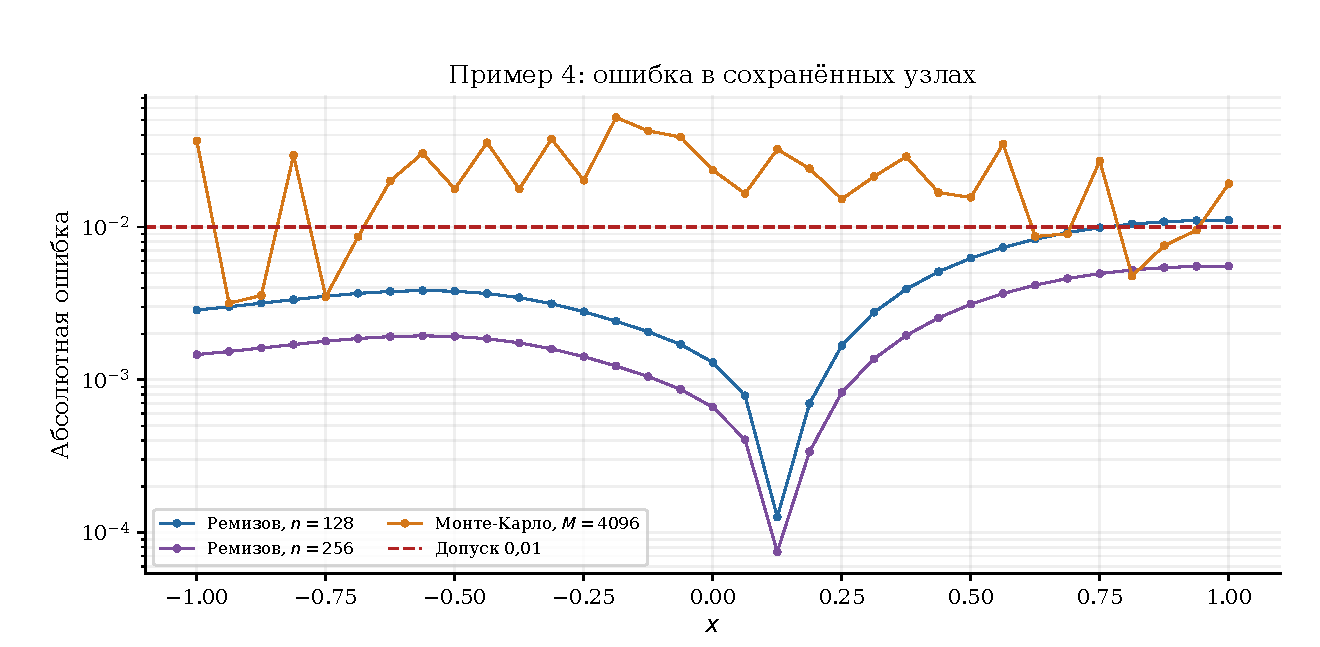
\includegraphics[width=.94\linewidth]{figures/example_04_error.pdf}\captionof{figure}{Пример 4. Абсолютная ошибка по сохранённым численным значениям. Порог относится к максимуму по 33 узлам; поведение ошибки между узлами не установлено.}\label{fig:example_04_error}\end{minipage}\end{center}

\clearpage

\subsection*{Б.5. Пример 5}\label{app:graphs5}

Полная дифференциальная постановка и числовые результаты приведены в п.~А.5. Сначала сопоставлены коэффициенты и точное решение на носителе.

\begin{center}\begin{minipage}{\linewidth}\centering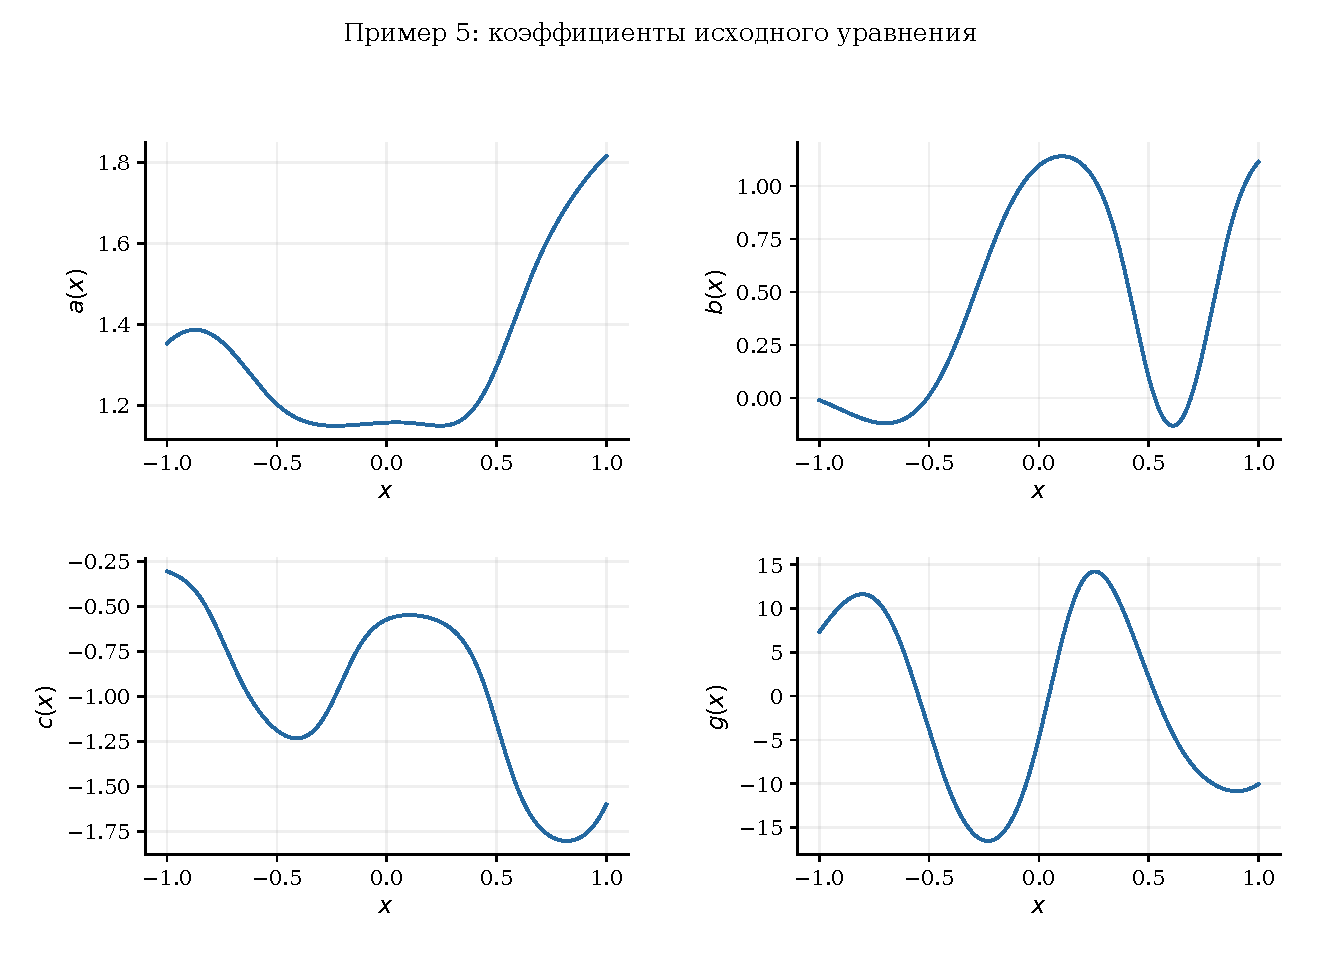
\includegraphics[width=.94\linewidth]{figures/example_05_coefficients.pdf}\captionof{figure}{Пример 5. Коэффициенты исходного уравнения на отрезке сравнения. Показан c(x), а не коэффициент $c_R(x)$ оператора. Все функции вычислены по сохранённым аналитическим определениям.}\label{fig:example_05_coefficients}\end{minipage}\end{center}

\begin{center}\begin{minipage}{\linewidth}\centering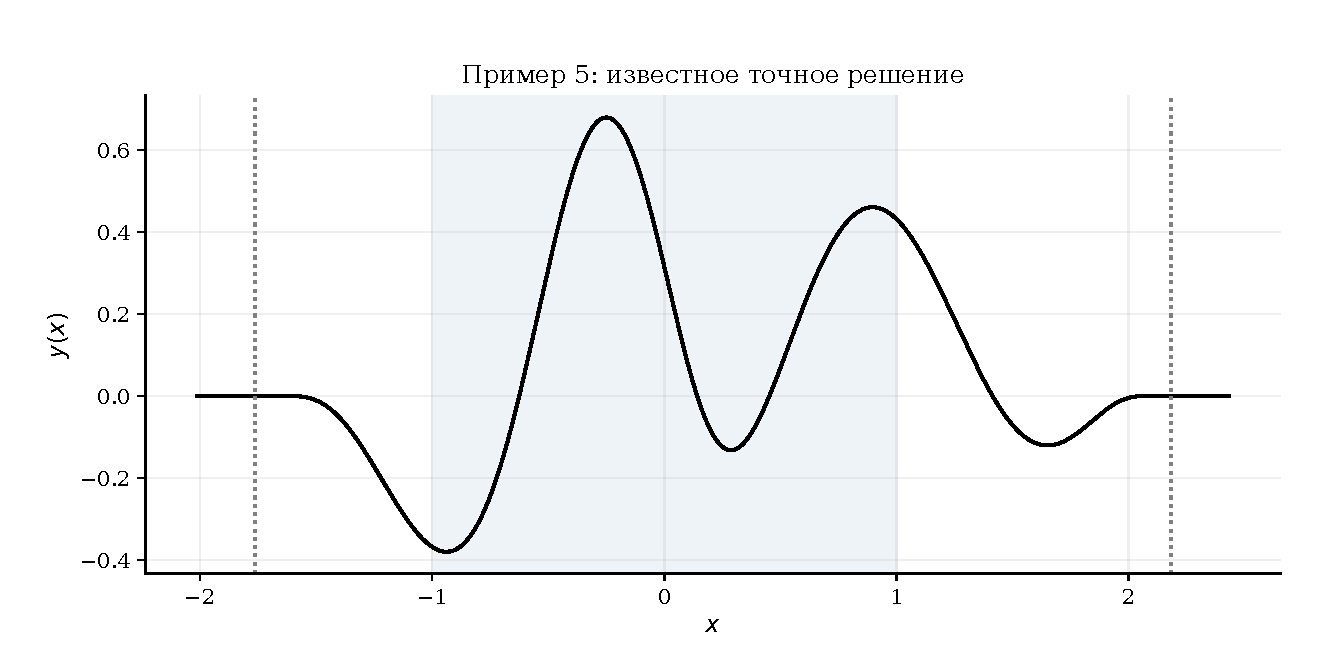
\includegraphics[width=.94\linewidth]{figures/example_05_exact.pdf}\captionof{figure}{Пример 5. Аналитическое решение на носителе и прилегающих участках прямой. Закрашен отрезок $[-1,1]$, на котором сохранены численные решения; пунктиром отмечены границы носителя.}\label{fig:example_05_exact}\end{minipage}\end{center}

\clearpage

\noindent\textbf{Пример 5: численное приближение и его ошибка.}

Кривые решений на общем масштабе могут казаться совпадающими, поэтому ниже отдельно показана абсолютная ошибка; критерием является её максимум, а не видимое совпадение отдельных участков.

\begin{center}\begin{minipage}{\linewidth}\centering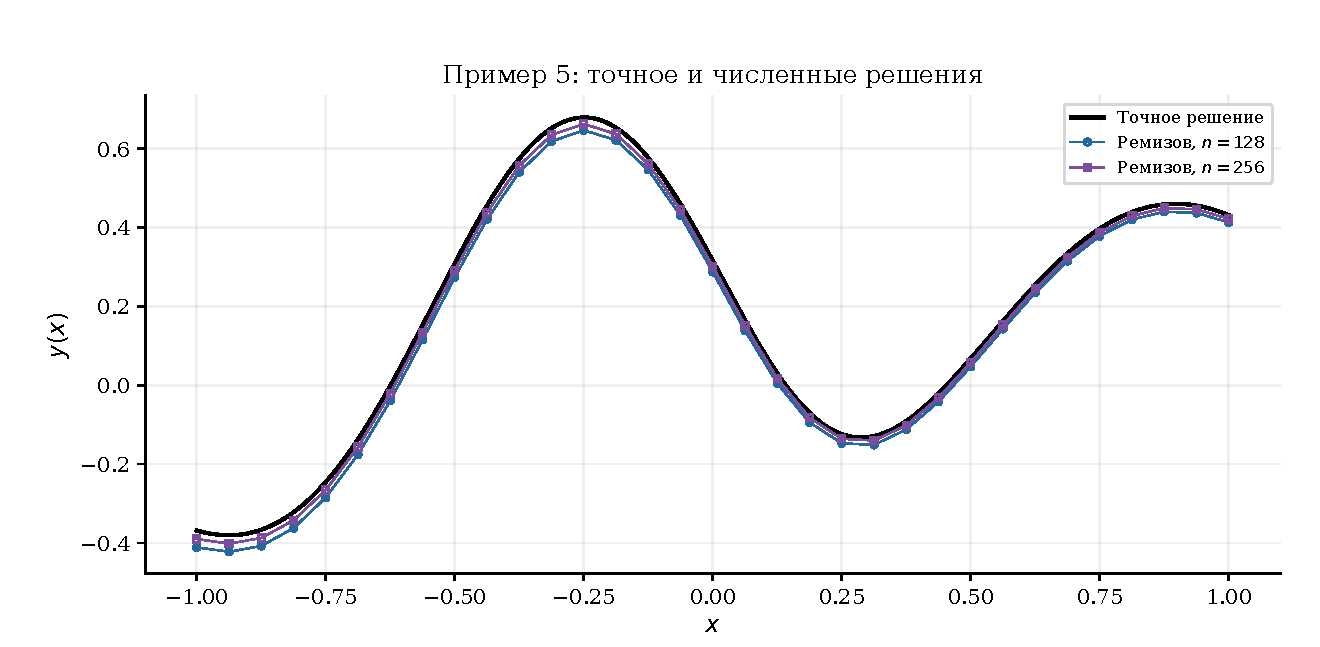
\includegraphics[width=.94\linewidth]{figures/example_05_solutions.pdf}\captionof{figure}{Пример 5. Точная кривая и сохранённые значения численных решений в 33 узлах. Отрезки между маркерами служат только для чтения. Новые численные значения между узлами не рассчитывались.}\label{fig:example_05_solutions}\end{minipage}\end{center}

\begin{center}\begin{minipage}{\linewidth}\centering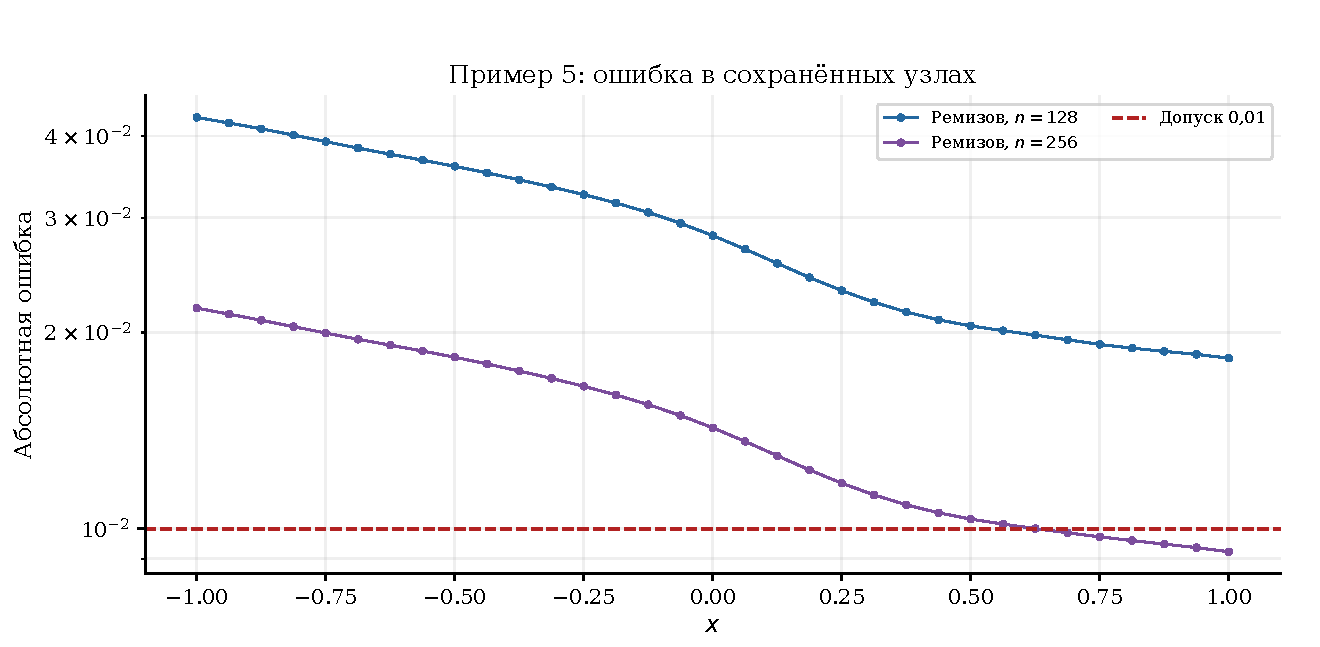
\includegraphics[width=.94\linewidth]{figures/example_05_error.pdf}\captionof{figure}{Пример 5. Абсолютная ошибка по сохранённым численным значениям. Порог относится к максимуму по 33 узлам; поведение ошибки между узлами не установлено.}\label{fig:example_05_error}\end{minipage}\end{center}

\clearpage

\subsection*{Б.6. Пример 6}\label{app:graphs6}

Полная дифференциальная постановка и числовые результаты приведены в п.~А.6. Сначала сопоставлены коэффициенты и точное решение на носителе.

\begin{center}\begin{minipage}{\linewidth}\centering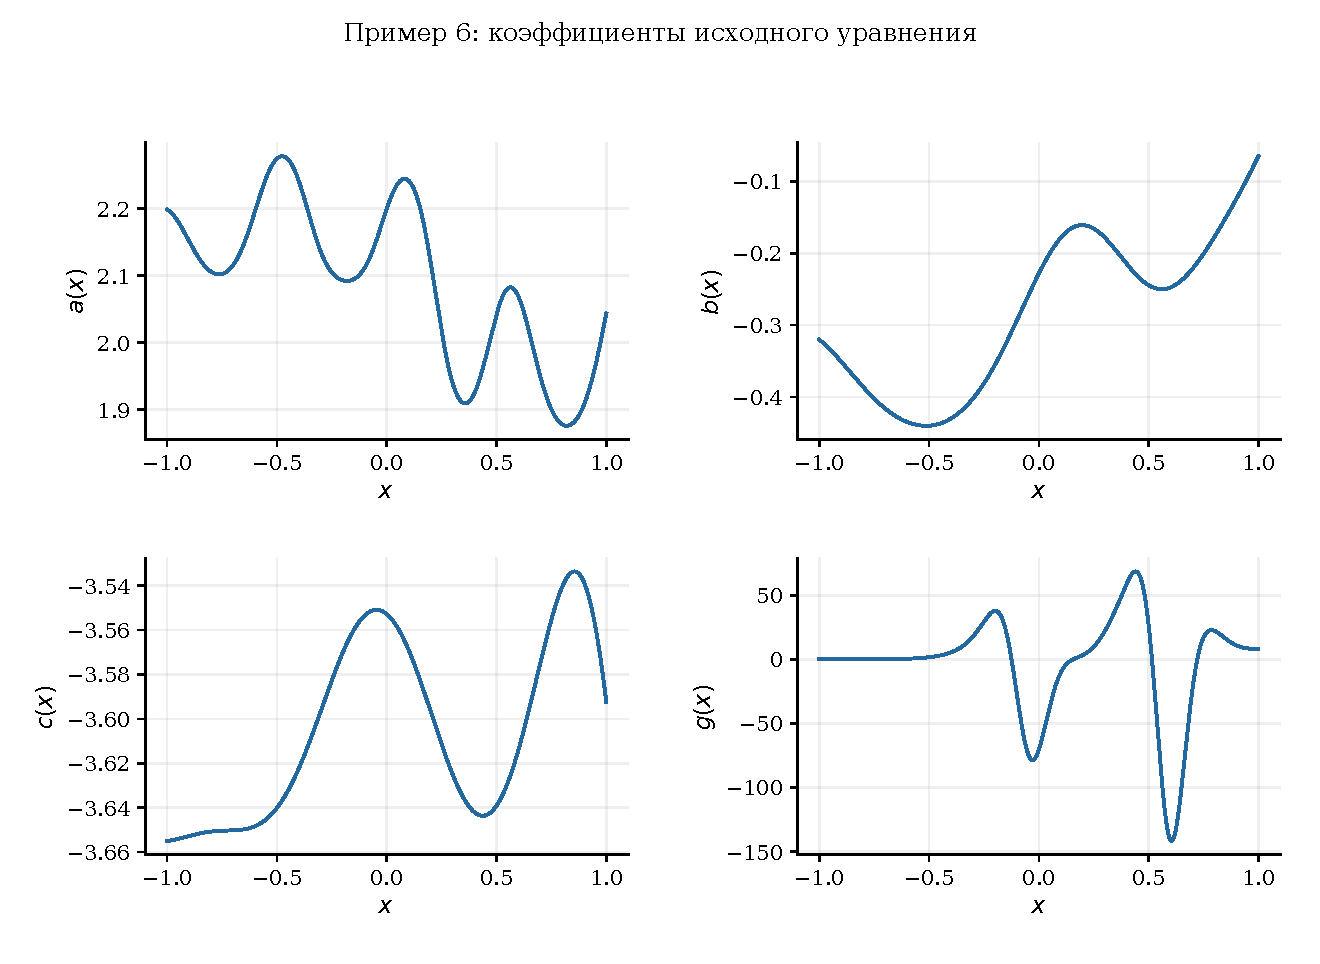
\includegraphics[width=.94\linewidth]{figures/example_06_coefficients.pdf}\captionof{figure}{Пример 6. Коэффициенты исходного уравнения на отрезке сравнения. Показан c(x), а не коэффициент $c_R(x)$ оператора. Все функции вычислены по сохранённым аналитическим определениям.}\label{fig:example_06_coefficients}\end{minipage}\end{center}

\begin{center}\begin{minipage}{\linewidth}\centering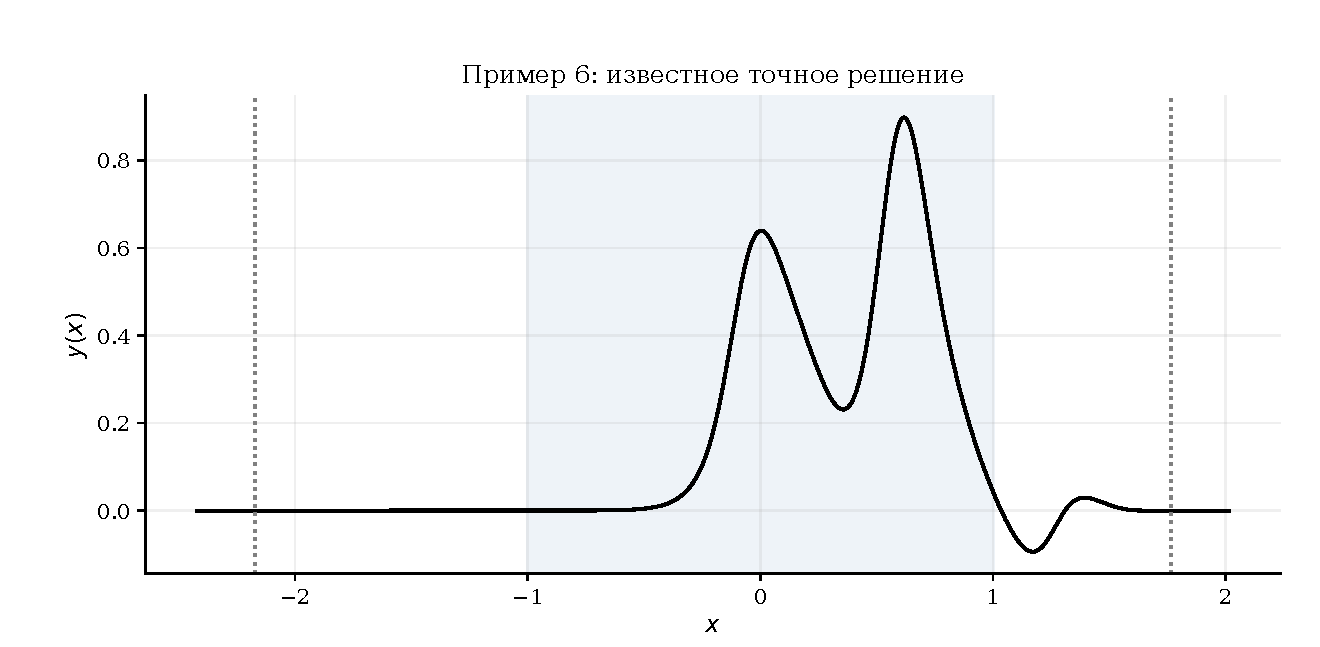
\includegraphics[width=.94\linewidth]{figures/example_06_exact.pdf}\captionof{figure}{Пример 6. Аналитическое решение на носителе и прилегающих участках прямой. Закрашен отрезок $[-1,1]$, на котором сохранены численные решения; пунктиром отмечены границы носителя.}\label{fig:example_06_exact}\end{minipage}\end{center}

\clearpage

\noindent\textbf{Пример 6: численное приближение и его ошибка.}

Кривые решений на общем масштабе могут казаться совпадающими, поэтому ниже отдельно показана абсолютная ошибка; критерием является её максимум, а не видимое совпадение отдельных участков.

\begin{center}\begin{minipage}{\linewidth}\centering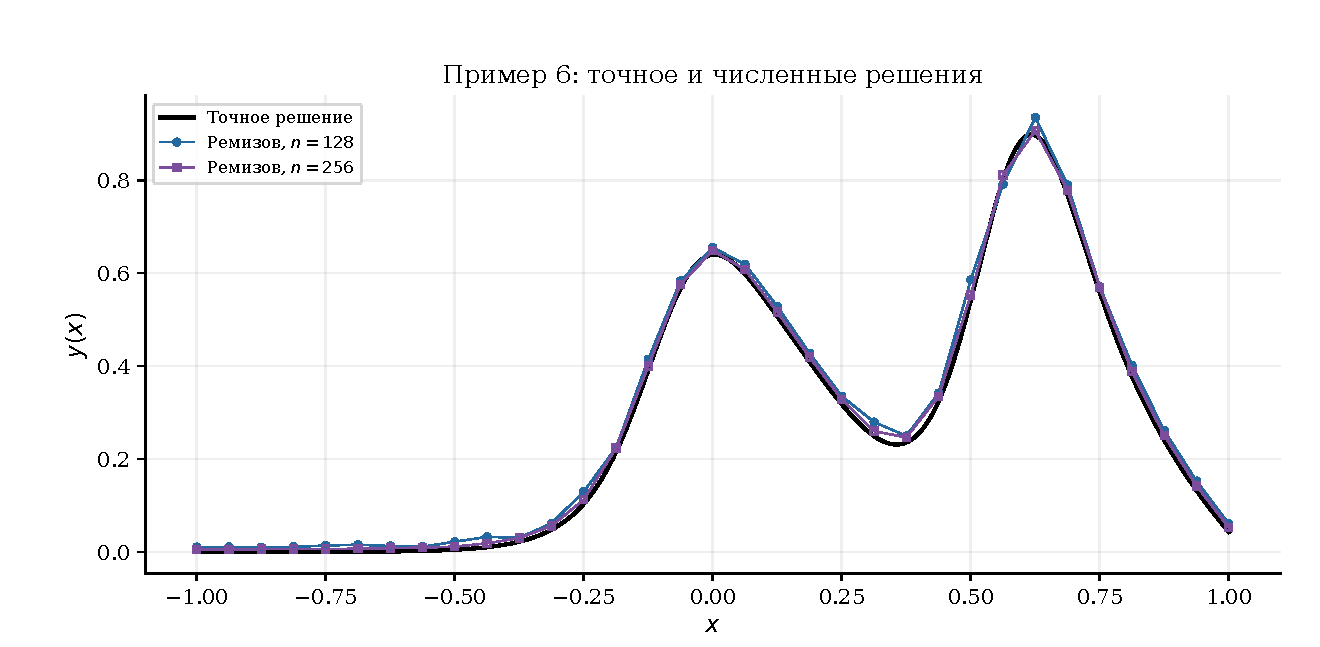
\includegraphics[width=.94\linewidth]{figures/example_06_solutions.pdf}\captionof{figure}{Пример 6. Точная кривая и сохранённые значения численных решений в 33 узлах. Отрезки между маркерами служат только для чтения. Новые численные значения между узлами не рассчитывались.}\label{fig:example_06_solutions}\end{minipage}\end{center}

\begin{center}\begin{minipage}{\linewidth}\centering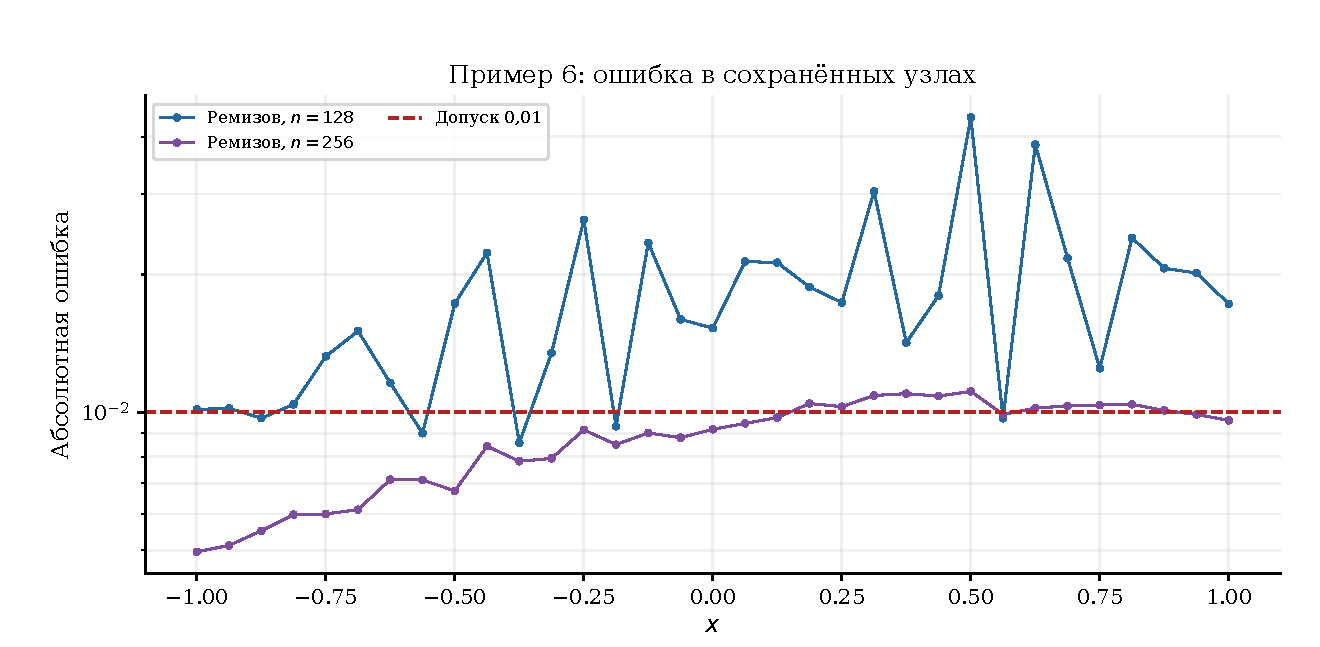
\includegraphics[width=.94\linewidth]{figures/example_06_error.pdf}\captionof{figure}{Пример 6. Абсолютная ошибка по сохранённым численным значениям. Порог относится к максимуму по 33 узлам; поведение ошибки между узлами не установлено.}\label{fig:example_06_error}\end{minipage}\end{center}

\clearpage

\subsection*{Б.7. Пример 7}\label{app:graphs7}

Полная дифференциальная постановка и числовые результаты приведены в п.~А.7. Сначала сопоставлены коэффициенты и точное решение на носителе.

\begin{center}\begin{minipage}{\linewidth}\centering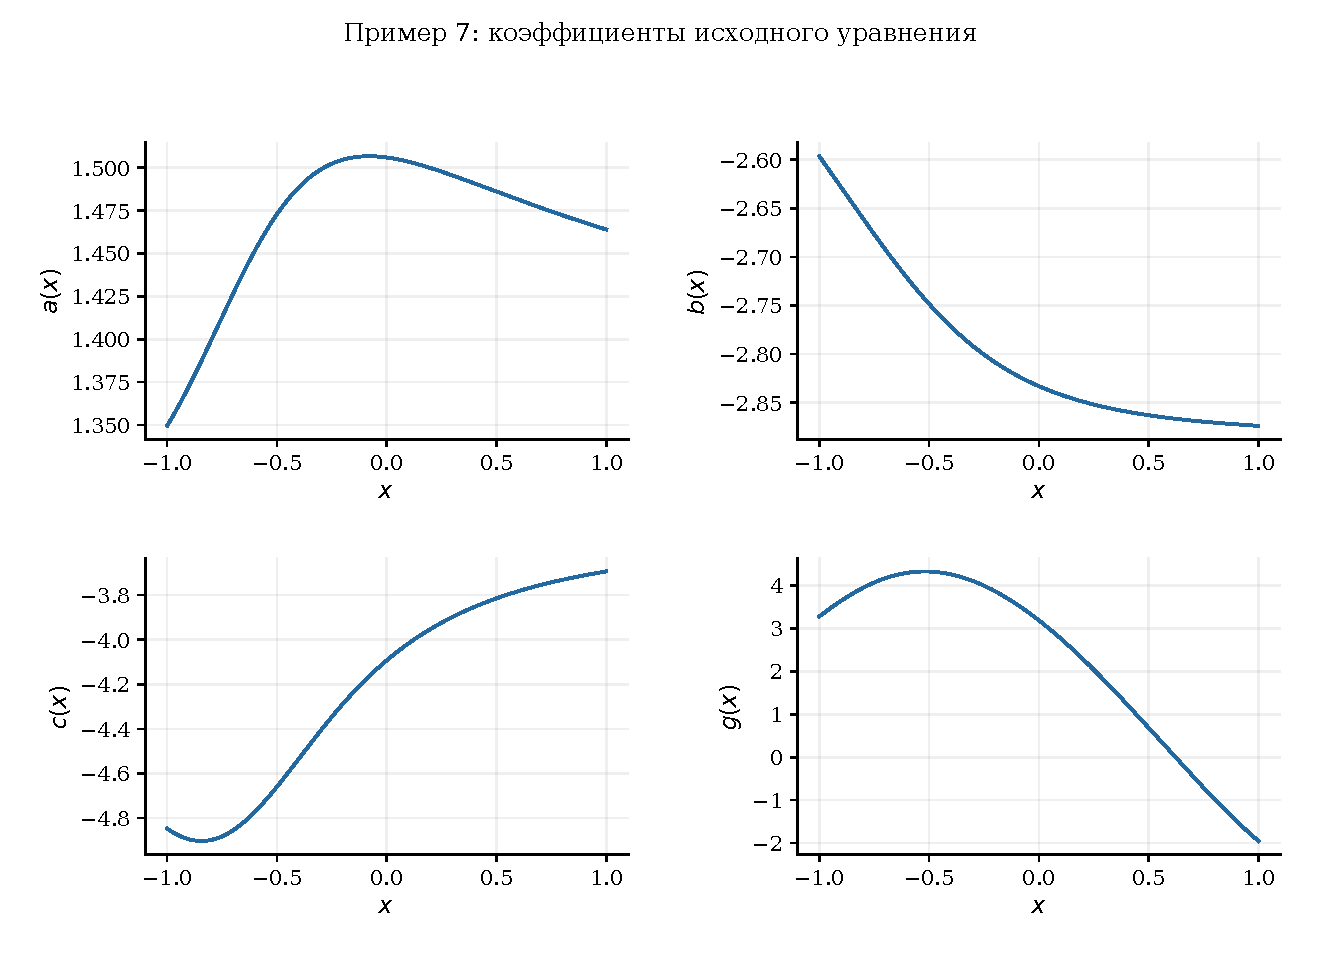
\includegraphics[width=.94\linewidth]{figures/example_07_coefficients.pdf}\captionof{figure}{Пример 7. Коэффициенты исходного уравнения на отрезке сравнения. Показан c(x), а не коэффициент $c_R(x)$ оператора. Все функции вычислены по сохранённым аналитическим определениям.}\label{fig:example_07_coefficients}\end{minipage}\end{center}

\begin{center}\begin{minipage}{\linewidth}\centering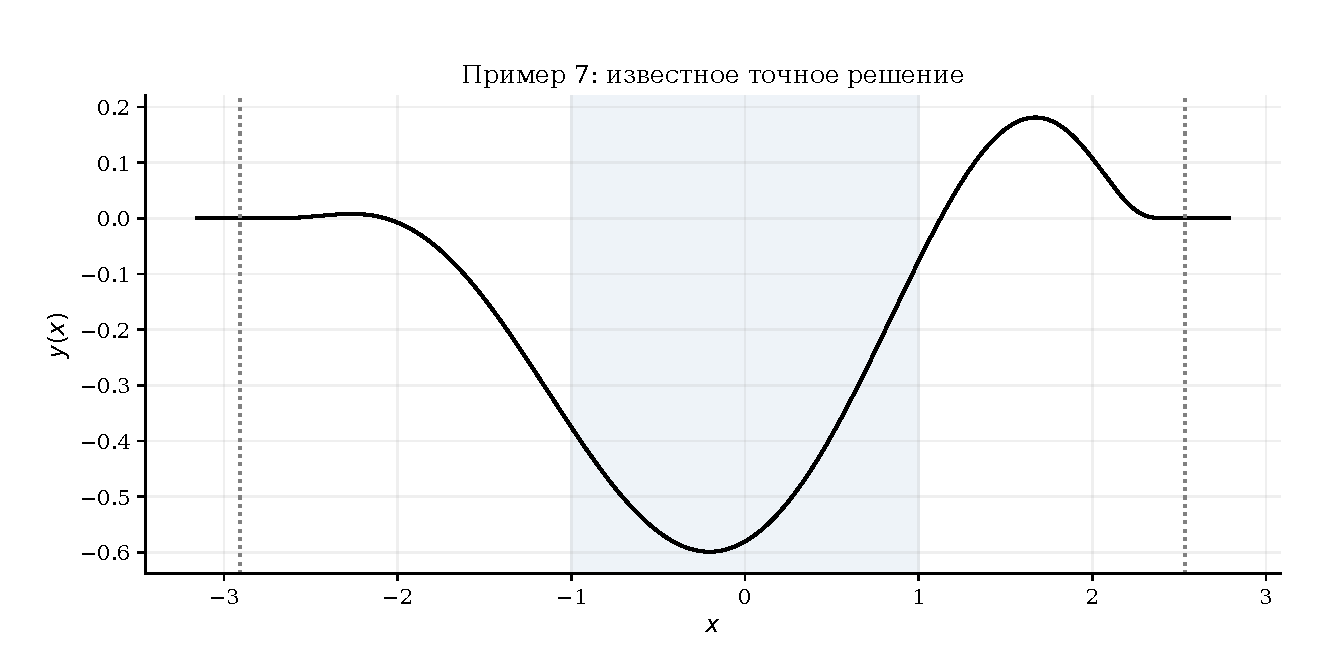
\includegraphics[width=.94\linewidth]{figures/example_07_exact.pdf}\captionof{figure}{Пример 7. Аналитическое решение на носителе и прилегающих участках прямой. Закрашен отрезок $[-1,1]$, на котором сохранены численные решения; пунктиром отмечены границы носителя.}\label{fig:example_07_exact}\end{minipage}\end{center}

\clearpage

\noindent\textbf{Пример 7: численное приближение и его ошибка.}

Кривые решений на общем масштабе могут казаться совпадающими, поэтому ниже отдельно показана абсолютная ошибка; критерием является её максимум, а не видимое совпадение отдельных участков.

\begin{center}\begin{minipage}{\linewidth}\centering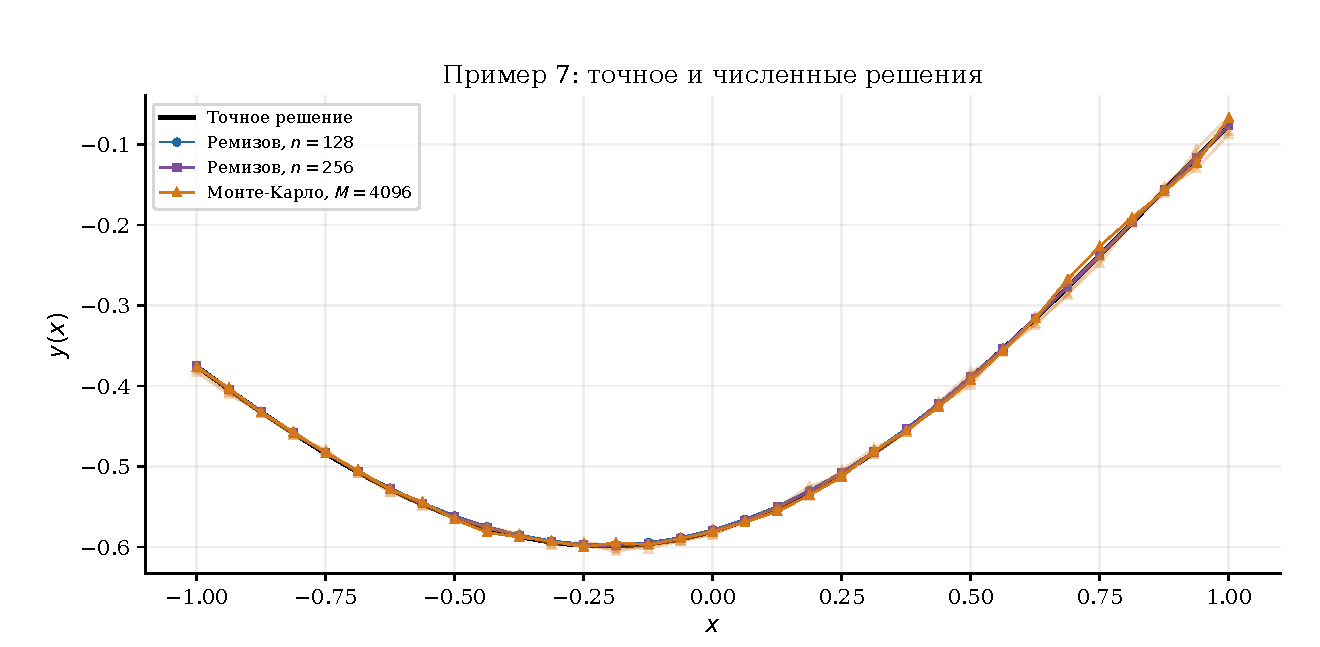
\includegraphics[width=.94\linewidth]{figures/example_07_solutions.pdf}\captionof{figure}{Пример 7. Точная кривая и сохранённые значения численных решений в 33 узлах. Отрезки между маркерами служат только для чтения. Тонкие линии показывают остальные реализации Монте-Карло; усреднение не выполнено.}\label{fig:example_07_solutions}\end{minipage}\end{center}

\begin{center}\begin{minipage}{\linewidth}\centering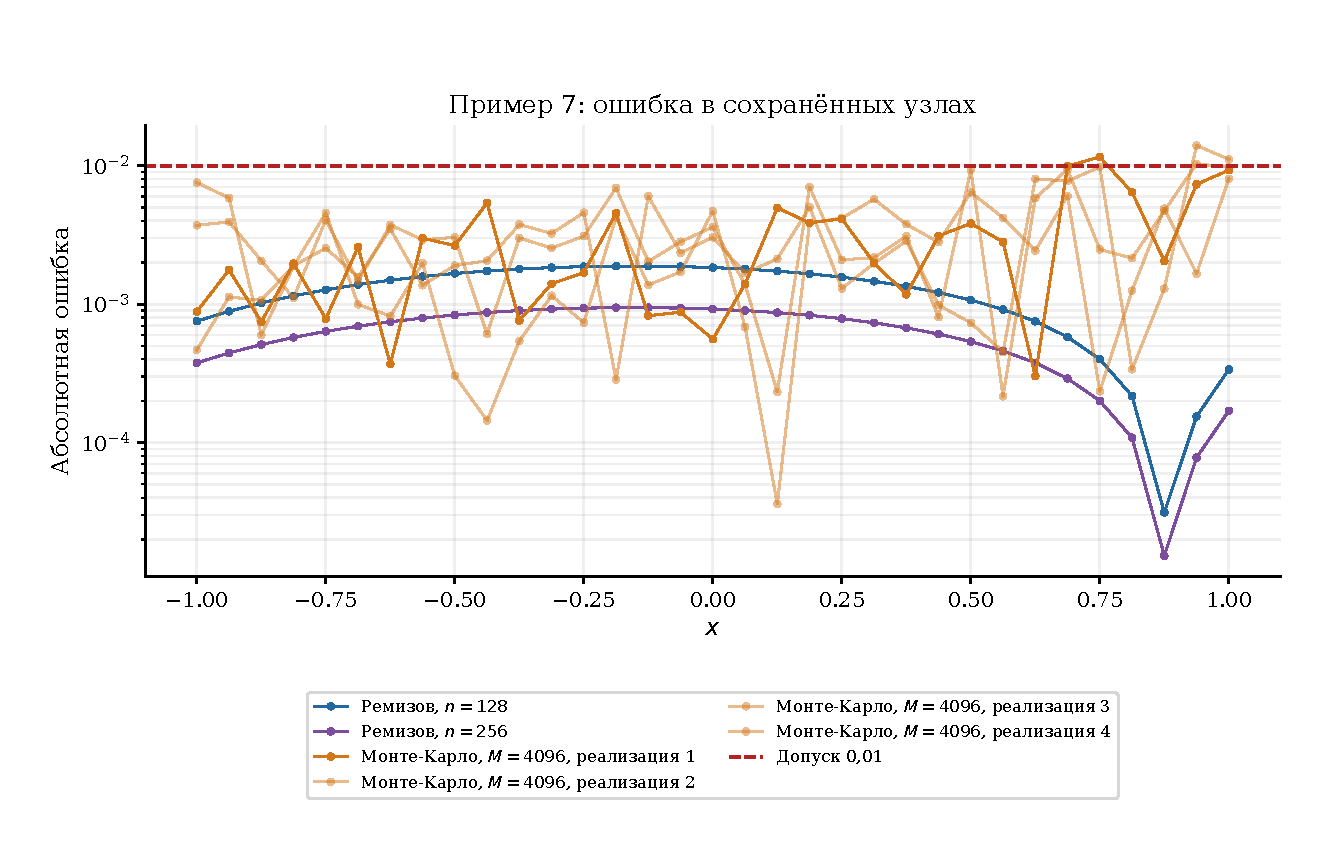
\includegraphics[width=.94\linewidth]{figures/example_07_error.pdf}\captionof{figure}{Пример 7. Абсолютная ошибка по сохранённым численным значениям. Порог относится к максимуму по 33 узлам; поведение ошибки между узлами не установлено.}\label{fig:example_07_error}\end{minipage}\end{center}

\clearpage

\noindent\textbf{Исторический опыт: четыре реализации на одном уравнении.}

\begin{center}\begin{minipage}{\linewidth}\centering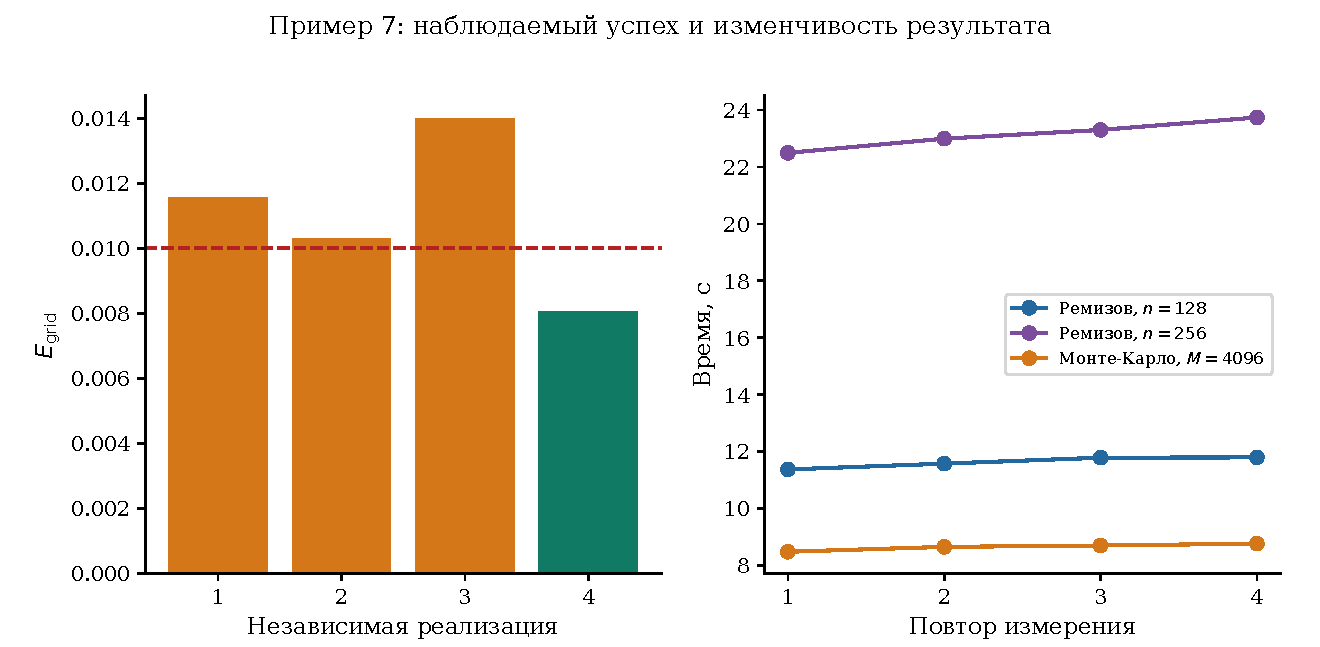
\includegraphics[width=.94\linewidth]{figures/example_07_repeats.pdf}\captionof{figure}{Один из четырёх Монте-Карло-ответов точен и быстрее метода Ремизова при n=128; три других нарушают допуск. Четыре реализации не подтверждают высокую надёжность следующего запуска. Опыт не включён в финальные 60 семейств.}\label{fig:example_07_repeats}\end{minipage}\end{center}

На этом уравнении все четыре повтора Ремизова при $n=128$ точны. Монте-Карло быстрее в данном временном блоке, но достигает допуска лишь в одном из четырёх ответов: $E=0{,}00804326$ против $0{,}01155969$, $0{,}01030280$ и $0{,}01399365$ в остальных. Среднее этих ответов не подставлено вместо каждой отдельной реализации.

Четыре реализации относятся к одному уравнению, а не к четырём независимым семействам. Этот пример сознательно выбран для обсуждения изменчивости и не является новой независимой проверкой модели. Его единственный точный стохастический ответ не добавляется к финальным $0/20$.
